\chapter{Background}
\label{chap:background}

In questo capitolo viene presentato il quadro teorico e tecnologico della tesi. La \cref{sec:comunicazioni_marittime_e_ais} analizza i sistemi di comunicazione marittima convenzionali (con focus sull'\ac{AIS}), evidenziando la differenza tra la loro banda limitata e l'elevata quantità di dati generata dalle navi a guida autonoma (\ac{MASS})~\cite{11217861, roadmap}.

Per superare questo limite, la \cref{sec:programmazione_aggregata_scr_collektive} introduce l'Aggregate Programming e il pattern \ac{SCR} (tramite il framework Collektive). In un ambiente marittimo, caratterizzato da un'elevata mobilità delle navi e connettività sparsa, questi approcci risultano efficaci poiché permettono di affrontare tali sfide creando protocolli di comunicazione resilienti e in grado di auto-organizzarsi dinamicamente~\cite{beal2015aggregate, casadei2019self, 11217861}.

Infine, la \cref{sec:simulazione_ambito_marittimo} illustra il ruolo del Modeling \& Simulation tramite il simulatore Alchemist. Poiché i test sul campo comportano limiti fisici ed elevati costi operativi, la simulazione offre l'ambiente virtuale ideale per sviluppare e valutare le prestazioni di tali reti cooperative~\cite{11217861, pianini_2013}.

\section{Comunicazioni marittime e AIS}
\label{sec:comunicazioni_marittime_e_ais}

Le comunicazioni marittime si basano su una combinazione di sistemi radio \ac{VHF} e satellitari (\ac{SatCom}) per garantire la sicurezza della navigazione e l'efficienza delle operazioni~\cite{11217861}. Mentre i sistemi satellitari assicurano una copertura globale, (comportando latenze e costi maggiori), i sistemi \ac{VHF} supportano lo scambio di dati a corto raggio (in linea di vista o Line of Sight, tipicamente a 40 km a seconda del meteo) per i collegamenti sia tra imbarcazioni (\ac{S2V}) sia verso le stazioni costiere (\ac{S2S})~\cite{11217861}. Una delle tecnologie fondamentali basate sui sistemi radio è l'\ac{AIS}. L'\ac{AIS} è un sistema di identificazione automatica che permette alle navi di trasmettere e ricevere in modo continuo informazioni sulla propria posizione, rotta, velocità e stato di navigazione, utilizzando la banda radio \ac{VHF} dedicata~\cite{itu_m1371_6}.

\subsection{Funzionamento del sistema AIS}
\label{sec:funzionamento_ais}

L'\ac{AIS} è nato come strumento per aumentare la sicurezza in mare, affiancando i radar per ridurre il rischio di collisioni e migliorare la ``consapevolezza situazionale" dei comandanti~\cite{itu_m1371_6, solas_mtsa_2015}. Ogni transponder \ac{AIS} invia periodicamente messaggi brevi (tipicamente ogni 2--6 secondi) che includono sia dati statici (identificativo \ac{IMO}, \ac{MMSI}, tipo di nave, dimensioni) sia dati dinamici (posizione \ac{GPS}, rotta, velocità, stato di navigazione), oltre a dati di viaggio come la destinazione prevista~\cite{itu_m1371_6}. Questi messaggi possono essere letti da altri transponder a bordo (modalità \ac{S2V}) e da stazioni costiere (\ac{S2S}), permettendo il monitoraggio del traffico da parte delle autorità (\ac{VTS}, Guardia Costiera)~\cite{itu_m1371_6, solas_mtsa_2015} e anche da servizi commerciali (es. portali come MarineTraffic\footnote{\url{https://www.marinetraffic.com}} o VesselFinder\footnote{\url{https://www.vesselfinder.com}}). La portata tipica è di alcune decine di miglia nautiche, limitata dalla propagazione \ac{VHF} e dalle condizioni meteorologiche~\cite{11217861}, ma può essere estesa tramite reti satellitari \ac{AIS-sat}~\cite{itu_m1371_6}.

\subsection{Struttura e codifica del messaggio AIS}
\label{sec:struttura_messaggio_ais}

I messaggi \ac{AIS} non vengono trasmessi in chiaro come testo, ma sono codificati in formato binario compresso (utilizzando una codifica a 6 bit) per minimizzare l'occupazione della banda radio \ac{VHF}~\cite{itu_m1371_6}. I diversi tipi di messaggi (da 1 a 27) rispondono a specifiche esigenze; tra questi, i messaggi di Tipo 1, 2 e 3 sono i più frequenti e vengono impiegati dalle navi di Classe A per comunicare periodicamente i dati di posizione dinamica~\cite{itu_m1371_6}. La \cref{tab:struttura_ais} descrive dettagliatamente la ripartizione dei bit all'interno di un frame \ac{AIS} di Posizione standard.

\begin{table}[htbp]
\centering
\small
\begin{tabularx}{\textwidth}{c l >{\raggedright\arraybackslash}X}
\toprule
\textbf{Bit} & \textbf{Nome Campo} & \textbf{Descrizione} \\
\midrule
6  & Message ID & Identifica il tipo di messaggio (valori: 1, 2 o 3). \\
2  & Repeat Indicator & Numero di ripetizioni del messaggio. \\
30 & Source ID (\ac{MMSI}) & Codice univoco di 9 cifre della nave. \\
4  & Navigational Status & Stato della nave (es. 0 = in navigazione, 1 = all'ancora, 5 = ormeggiata). \\
8  & \ac{ROT} & Velocità di accostata (virata) a destra o sinistra. \\
10 & \ac{SOG} & Velocità rispetto al fondo (risoluzione 0.1 nodi). \\
1  & Position Accuracy & Accuratezza del \ac{GPS} (1 = alta, $\le 10 \text{ m}$; 0 = bassa, $> 10 \text{ m}$). \\
28 & Longitude & Longitudine in 1/10000 di minuto d'arco. \\
27 & Latitude & Latitudine in 1/10000 di minuto d'arco. \\
12 & \ac{COG} & Rotta rispetto al fondo (in decimi di grado, 0--3599). \\
9  & True Heading & Prua vera della nave (0--359 gradi). \\
6  & Time Stamp & Secondo della coordinata temporale \ac{UTC} di generazione (0--59). \\
2  & Special Manoeuvre & Indicatore di manovre speciali. \\
2  & Spare & Bit di riserva inutilizzati (impostati a 0). \\
1  & Transmit Power & Potenza di trasmissione. \\
1  & RAIM flag & Indicatore di integrità del ricevitore \ac{GPS}. \\
19 & Communication State & Dati di sincronizzazione e gestione degli slot temporali. \\
\midrule
\textbf{168} & \textbf{Totale} & Struttura che occupa 1 slot di trasmissione. \\
\bottomrule
\end{tabularx}
\caption{Struttura del payload di un messaggio \ac{AIS} di Posizione (Tipo 1, 2, 3).}
\label{tab:struttura_ais}
\end{table}
\newpage

\subsection{Aspetti normativi e applicazioni}
\label{sec:aspetti_normativi}

L'uso del Sistema di Identificazione Automatica è regolato dall'\ac{IMO} ed è obbligatorio ai sensi della convenzione \ac{SOLAS} per le navi commerciali in viaggio internazionale con stazza lorda pari o superiore a 300 \ac{GT}, e per tutte le navi passeggeri indipendentemente dalle loro dimensioni~\cite{10.1145/2664243.2664257, solas_mtsa_2015}. Oltre all'identificazione e al monitoraggio dei corridoi marittimi, l'\ac{AIS} è oggi impiegato in diversi ambiti. Tra questi spicca la prevenzione delle collisioni in tempo reale (\ac{CPA}), che permette ai sistemi di bordo di innescare allarmi visivi e acustici qualora si rilevi una possibile collisione~\cite{10.1145/2664243.2664257}. Inoltre, il sistema risulta fondamentale per le operazioni di ricerca e soccorso (\ac{SAR}) e la gestione di uomini in mare (\ac{MOB}): i trasmettitori di soccorso (es. \ac{AIS-SART}) si attivano a contatto con l'acqua trasmettendo la posizione \ac{GPS} a tutte le unità limitrofe, utilizzando messaggi specifici e un prefisso \ac{MMSI} dedicato~\cite{10.1145/2664243.2664257, itu_m1371_6}.
Un altro campo in cui viene utilizzato il Sistema di Identificazione Automatica è la segnalazione di ostacoli tramite ausili alla navigazione (\ac{AtoN}): boe, fari o stazioni possono trasmettere le proprie coordinate o simulare ostacoli virtuali (Virtual \ac{AtoN}) per deviare il traffico da aree pericolose o fondali bassi~\cite{10.1145/2664243.2664257, itu_m1371_6}. Infine, l'\ac{AIS} agevola il monitoraggio ambientale per rintracciare le navi responsabili di versamenti illegali di petrolio in mare~\cite{10.1145/2664243.2664257}.

\subsection{Limiti e problemi aperti}
\label{sec:limiti}

Nonostante l'ampia diffusione, sono presenti alcuni limiti e vulnerabilità dell'\ac{AIS}. In primo luogo, la sua natura non autenticata lo espone a vulnerabilità informatiche. I dati generati a bordo possono essere manipolati (\emph{spoofed}) per creare navi inesistenti o falsi allarmi \ac{SAR}/\ac{CPA}, alterati sovrascrivendo i segnali (\emph{hijacking}) oppure resi indisponibili tramite attacchi radio \emph{Denial of Service}, come il blocco del salto di frequenza (\emph{frequency hopping}) o l'esaurimento degli slot disponibili (\emph{slot starvation})~\cite{10.1145/2664243.2664257}. Dal punto di vista fisico, il canale della trasmissione \ac{VHF} offre una larghezza di banda molto stretta (circa 10 kbps) a fronte di una copertura limitata Line of Sight (tipicamente 40 km, fortemente dipendente dalle condizioni meteorologiche)~\cite{11217861}. Di conseguenza, le attuali reti risultano incompatibili con i requisiti delle navi a guida autonoma (\ac{MASS}): questi mezzi richiedono sensori avanzati come telecamere ad alta risoluzione, \ac{LiDAR} e radar, generando flussi di dati continui nell'ordine dei Mbps che le attuali reti marittime non sono in grado di sostenere~\cite{11217861}.

In particolare, questo lavoro di tesi affronterà l'ultimo problema elencato sopra, utilizzando la programmazione aggregata (\cref{sec:programmazione_aggregata_scr_collektive}).

\section{Aggregate Programming, SCR e Collektive}
\label{sec:programmazione_aggregata_scr_collektive}

\subsection{Programmazione Aggregata (AP)}
\label{sec:programmazione_aggregata}

La programmazione di sistemi distribuiti moderni, come l'\ac{IoT} o le reti navali, risulta complessa a causa dell'eterogeneità dei dispositivi, dei guasti frequenti e della necessità di interazioni basate sulla prossimità fisica~\cite{beal2015aggregate}. Per far fronte a questi problemi, \ac{AP} propone un cambio di paradigma: l'unità base della computazione non è più il singolo dispositivo, ma un intero insieme (o aggregato) di nodi cooperanti, astraendo dettagli come il numero e l'esatta posizione dei singoli apparati~\cite{beal2015aggregate, beal2016foundations}. 
\ac{AP} è un approccio di macro-programmazione funzionale basato sul concetto di campo computazionale (computational field), ovvero una struttura dati distribuita che mappa ogni dispositivo in un dato spazio e tempo a un valore~\cite{viroli2018engineering, 11217861}. I dispositivi eseguono tutti un medesimo programma in modo asincrono (in round continui) seguendo un modello a tre fasi~\cite{11217861}:
\begin{itemize} 
  \item \emph{sense}: il nodo raccoglie informazioni dall'ambiente locale e dai messaggi ricevuti dai vicini durante la fase di riposo;
  \item \emph{compute}: il programma aggregato viene valutato usando i dati raccolti, producendo un nuovo stato locale e i messaggi da condividere;
  \item \emph{share}: il dispositivo invia i messaggi ai propri vicini.
\end{itemize}

\subsection{Field Calculus (FC) e Building Blocks}
\label{sec:fc}

Il fondamento matematico di Aggregate Programming è \ac{FC}, un calcolo universale minimale che modella le interazioni dei dispositivi nello spazio e nel tempo~\cite{beal2016foundations, viroli2018engineering}. FC opera a un basso livello di astrazione, basandosi su un numero ridotto di costrutti~\cite{viroli2018engineering}:
\begin{itemize}
    \item \texttt{nbr} (\emph{Neighborhood values}): permette l'interazione del dispositivo con il vicinato, raccogliendo e mappando i valori più recenti di una determinata espressione provenienti dai nodi vicini e dal nodo stesso~\cite{viroli2018engineering, beal2014building};
    \item \texttt{rep} (\emph{Time evolution}): modella la dinamica temporale, inizializzando una variabile di stato locale e aggiornandola ciclicamente a ogni round di computazione~\cite{viroli2018engineering, beal2014building};
    \item \texttt{if} (\emph{Domain restriction}): partiziona la rete in sottoregioni in cui vengono eseguiti rami di codice differenti~\cite{viroli2018engineering}.
\end{itemize}
 
 Per aumentare il livello di astrazione ed evitare la gestione manuale dei costrutti come \texttt{rep} e \texttt{nbr}, come illustrato in \cref{fig:buildingBlocks}, sono stati identificati una serie di building blocks formalmente provati per essere auto-stabilizzanti. Questi blocchi incapsulano i costrutti di \ac{FC} e ciò garantisce che il sistema che li utilizza sia in grado di recuperare da guasti e adattarsi ai cambiamenti topologici, convergendo sempre verso lo stato corretto~\cite{beal2014building, viroli2018engineering}.
I principali operatori di base sono~\cite{beal2014building, beal2015aggregate}:
\begin{itemize}
  \item \textbf{G}: diffonde informazioni da una regione sorgente seguendo un gradiente (es. calcolo delle distanze minime o broadcast);
  \item \textbf{C}: accumula informazioni muovendosi lungo il gradiente di un potenziale (tipicamente verso un nodo pozzo o sink);
  \item \textbf{T}: regola l'evoluzione temporale, agendo come una memoria a tempo o un count-down;
  \item \textbf{S}: elegge dei leader locali in modo sparso, frammentando lo spazio in partizioni (es. diagrammi di Voronoi).
\end{itemize}
\begin{figure}
    \centering
    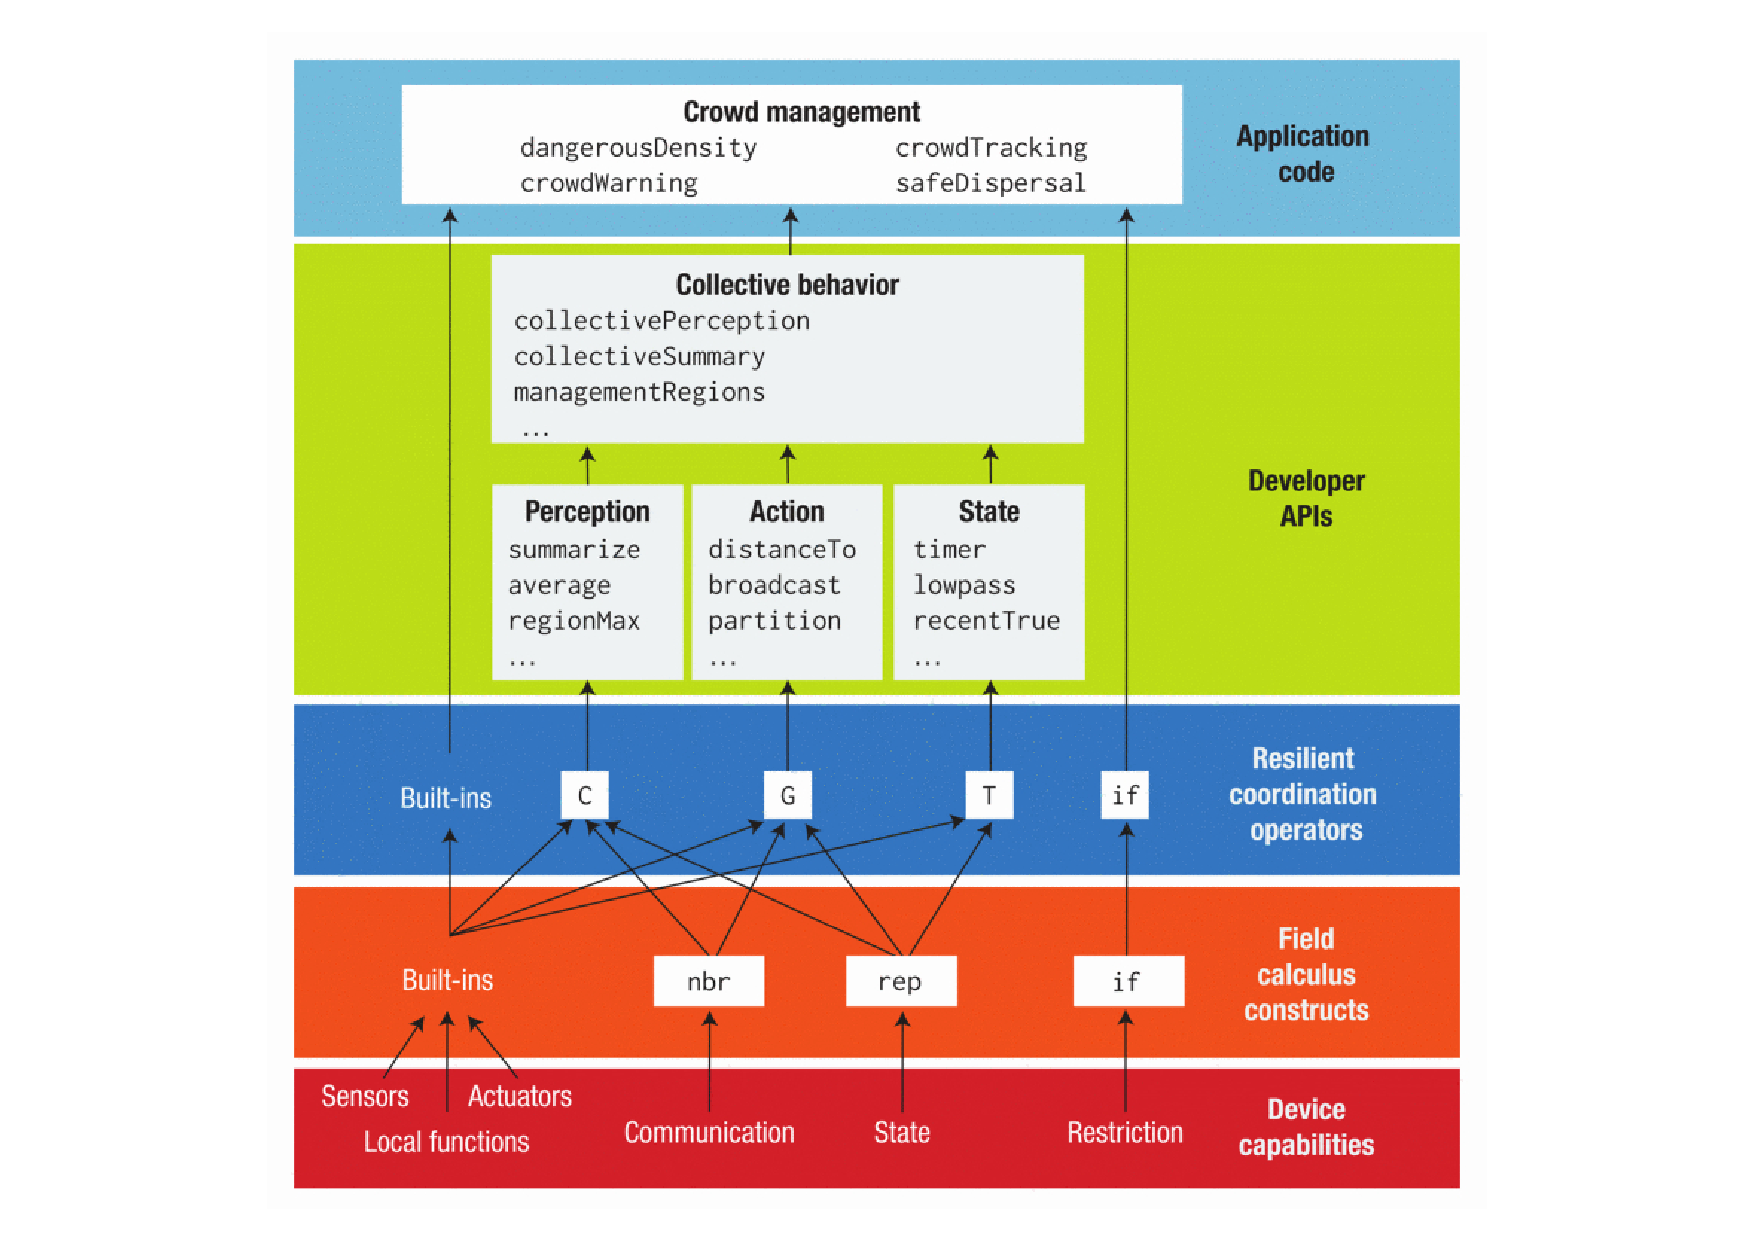
\includegraphics[width=\linewidth]{figures/imgBuildingBlocks.pdf}
    \caption{Livelli di astrazione della programmazione aggregata. Le capacità software e hardware di alcuni dispositivi sono utilizzate per implementare costrutti di \ac{FC} a livello aggregato. Questi costrutti sono utilizzati per implementare operazioni di coordinamento a blocchi resilienti, che vengono poi racchiuse e combinate insieme per produrre API. © 2015 IEEE. Ristampata, con permesso, da~\cite{beal2015aggregate}.}
    \label{fig:buildingBlocks}
\end{figure}
\newpage

\subsection{Self-organising Coordination Regions (SCR)}
\label{sec:scr}

Sfruttando i building blocks, è stato ideato un design pattern chiamato \ac{SCR}, pensato appositamente per gestire reti molto grandi e complesse, come quelle dell'Edge Computing~\cite{casadei2019self}. Il suo obiettivo è trovare un compromesso efficace tra un controllo totalmente centralizzato e uno completamente decentralizzato~\cite{casadei2019self}. Il sistema si auto-organizza suddividendosi spontaneamente in regioni. All'interno di ciascuna regione, le attività vengono coordinate in modo autonomo grazie a un continuo scambio di informazioni (un ciclo di feedback, come mostrato in \cref{fig:scr}) tra un nodo responsabile (leader) e i dispositivi circostanti~\cite{casadei2019self}. Il funzionamento di questo pattern si basa su quattro processi continui~\cite{casadei2019self}:
\begin{enumerate}
  \item \emph{Elezione dei leader}: vengono eletti i leader da un insieme di candidati (tramite l'operatore S).
  \item \emph{Formazione delle regioni}: ogni nodo viene assegnato a un singolo leader, costruendo i percorsi di comunicazione ottimali.
  \item \emph{Raccolta delle informazioni}: flussi di dati si muovono dai nodi della regione verso il leader, utilizzando algoritmi come C.
  \item \emph{Propagazione delle informazioni}: i leader valutano i dati raccolti e diffondono i risultati o le direttive verso tutti i membri della propria regione (utilizzando G).
\end{enumerate}
Il pattern \ac{SCR} è resiliente: se un leader subisce un guasto o si verificano variazioni nel carico, il sistema riconfigura automaticamente i leader e ridimensiona le regioni in pochi secondi~\cite{casadei2019self}.
\begin{figure}
    \centering
    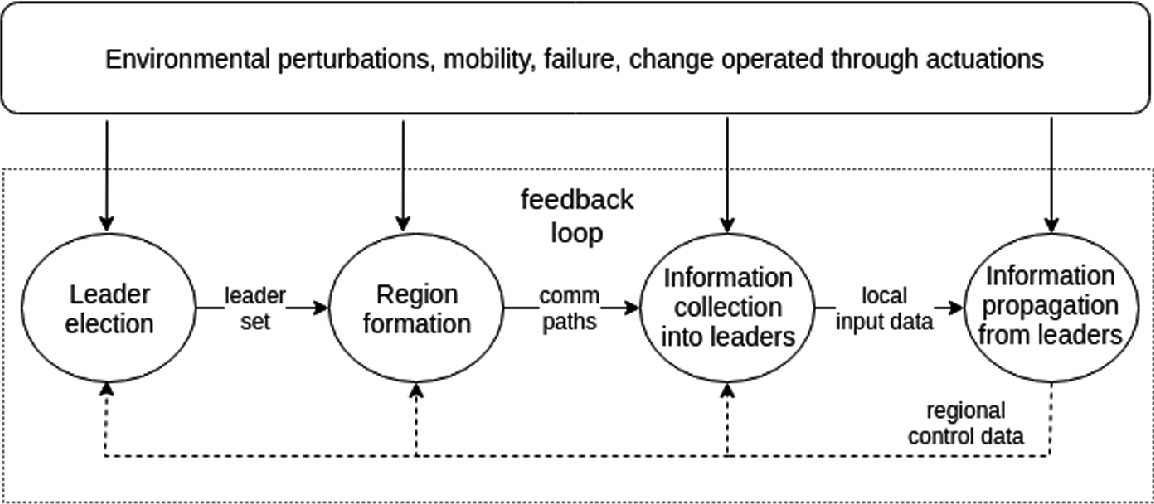
\includegraphics[width=\linewidth]{figures/SCR.png}
    \caption{Prospettiva dinamica di \ac{SCR}~\cite{casadei2019self}.}
    \label{fig:scr}
\end{figure}
\newpage

\subsection{Collektive}
\label{sec:collektive}

Dal punto di vista dell'implementazione, la programmazione aggregata viene concretizzata tramite \ac{DSL}, tra cui ScaFi\footnote{\url{https://scafi.github.io/}} (basato su Scala) e Protelis\footnote{\url{https://protelis.github.io/wiki-beta/}} (basato su Java). In questa tesi viene utilizzato \textbf{Collektive}\footnote{\url{https://collektive.github.io}}, un \ac{DSL} nativo basato su Kotlin.
È un framework open-source progettato per semplificare lo sviluppo di sistemi distribuiti attraverso l'utilizzo dei principi di \ac{AP}~\cite{collektiveWeb}.
Architetturalmente, Collektive è suddiviso in tre macro-componenti:
\begin{enumerate}
  \item un plugin per il compilatore, che si occupa di gestire l'allineamento;
  \item il \ac{DSL}, che definisce i costrutti linguistici fondamentali;
  \item e la libreria standard, che fornisce le funzioni essenziali per \ac{AP}.
\end{enumerate}

Il \ac{DSL} Collektive espone funzioni per la gestione dello stato e delle interazioni di rete, ad esempio~\cite{11217861}:
\begin{itemize}
  \item \texttt{neighboring}: consente di osservare e mappare in un campo i valori di una specifica variabile nei nodi vicini. Corrisponde a nbr in \ac{FC};
  \item \texttt{exchange}: è uno degli operatori più importanti del \ac{DSL}. Modella la comunicazione \emph{anisotropica}, consentendo a un nodo di inviare messaggi differenti a vicini diversi.
  \item \texttt{share}: modella la comunicazione \emph{isotropica} (invia lo stesso stato a tutti), combinando lo stato precedente con le informazioni scambiate nel vicinato per evolvere i dati nello spazio e nel tempo;
  \item \texttt{evolve}: equivale a \texttt{rep} nel \ac{FC} e consente di modellare l'evoluzione dello stato del dispositivo nel tempo;
  \item \texttt{alignedOn}: introduce la segmentazione del dominio (domain segmentation), isolando le comunicazioni ed eseguendo i blocchi di codice esclusivamente tra i dispositivi che soddisfano e condividono un medesimo identificatore (pivot)~\cite{11217861}.
\end{itemize}

I building blocks vengono implementati componendo queste primitive. Operazioni come \texttt{gradientCast} o il calcolo delle distanze tramite Bellman-Ford si ottengono combinando \texttt{exchange} o \texttt{share} con una metrica, ad esempio calcolando la formula di Haversine sui dati \ac{GPS} recuperati tramite \texttt{neighboring}~\cite{11217861}.

Per quanto concerne l'implementazione del pattern \ac{SCR}, Collektive vi provvede utilizzando algoritmi di elezione e segmentazione. La formazione dinamica delle regioni è delegata alla funzione \texttt{boundedElection}, che partiziona la rete senza alcuna coordinazione centrale~\cite{11217861}. L'algoritmo riceve in input il diametro massimo del cluster e una metrica di ``forza" del nodo (la priorità del candidato).
Questa ``forza" coincide con l'eleggibilità del dispositivo a diventare leader (che può basarsi su risorse energetiche, di calcolo, o sul data rate come nel caso dell'esperimento iniziale di questa tesi~\cite{11217861}). È possibile personalizzare l'elezione del leader utilizzando \texttt{Candidacy} (rappresenta la candidatura in un'elezione di un candidato) all'interno del parametro \texttt{selectBest} in \texttt{boundedElection}. Valutando le ``forze", \texttt{boundedElection} risolve le contese ed elegge i leader, adattandosi tempestivamente ai guasti o ai cambiamenti topologici~\cite{11217861}. 
Una volta eletti i leader, all'interno della regione viene utilizzato l'operatore \texttt{alignedOn(leader)}: in questo modo i dispositivi di una stessa regione restringono il proprio dominio alla sola regione di appartenenza, instaurando canali diretti (come dei \texttt{convergeCast}) per instradare le informazioni senza interferire con le regioni adiacenti~\cite{11217861}.
\texttt{temperatureEntrypoint} (\cref{lst:exampleCollektive}) rappresenta un esempio di un semplice algoritmo in cui vengono utilizzate le nozioni di \ac{SCR} e \ac{AP}: i nodi possiedono un attributo ``temperatura". Essi si organizzano in regioni con il proprio leader e quest’ultimo si occupa di calcolare la media delle temperature dei dispositivi della propria area. Se la media supera i 30°C allora il leader diffonde un allarme.
\lstinputlisting[
float,
language=Kotlin,
label={lst:exampleCollektive},
caption={Esempio di codice Collektive per una semplice simulazione di programmazione aggregata.}
]{listings/exampleCollektive.kt}
\newpage

\section{Simulazione in ambito marittimo}
\label{sec:simulazione_ambito_marittimo}

\subsection{Modeling \& Simulation (M\&S)}
\label{sec:ms}

I porti marini e gli scenari di navigazione costiera sono sistemi altamente complessi, caratterizzati da un'elevata densità di traffico, condizioni meteo variabili e diversi attori (navi mercantili, piccoli natanti, rimorchiatori, e torri di controllo). In tale contesto, testare nuove configurazioni di rete, valutare l'efficienza delle operazioni o formare il personale sul campo risulta spesso proibitivo per questioni di sicurezza, limiti fisici ed elevati costi operativi~\cite{chiurco_phd}. 

Per risolvere queste problematiche, il paradigma \ac{MS} rappresenta lo strumento d'eccellenza. \ac{MS} consente di riprodurre il comportamento del sistema reale attraverso un modello computazionale, offrendo un ambiente virtuale in cui analizzare scenari ``what-if", condurre analisi sugli incidenti e massimizzare l'efficacia del training~\cite{chiurco_phd}. In particolare, la simulazione distribuita permette l'addestramento congiunto di piloti di navi e operatori del traffico (\ac{VTS}) all'interno di un unico ambiente virtuale condiviso, riducendo i rischi e i costi associati agli errori in fase di apprendimento~\cite{chiurco_phd}. Oltre alla formazione del personale, la simulazione si rivela oggi un mezzo fondamentale per lo sviluppo e la prototipazione di reti di telecomunicazione e schemi di coordinamento adattivo destinati alle future navi a guida autonoma (\ac{MASS})~\cite{11217861, chiurco_phd}.

\subsection{Alchemist}
\label{sec:alchemist}

Per l'esecuzione e la valutazione dell'esperimento di questa tesi è stato adottato \textbf{Alchemist}\footnote{\url{https://alchemistsimulator.github.io/}}, una piattaforma di simulazione di sistemi distribuiti, particolarmente adatta alla programmazione aggregata. Consente di modellare e simulare le interazioni tra agenti in ambienti complessi, supportando diverse astrazioni e paradigmi di programmazione~\cite{collektiveWeb}.

\subsubsection{Meta-modello e Astrazioni}
\label{sec:metamodello}

Per garantire la flessibilità necessaria a simulare scenari complessi, la logica di Alchemist, come mostrato in \cref{fig:AlchemistMetaModel}, si basa su un meta-modello le cui entità fondamentali sono~\cite{pianini_2021}:
\begin{itemize}
    \item \emph{Environment}: lo spazio in cui vivono i nodi, con la responsabilità di mapparne la posizione. Può includere ostacoli fisici, mappe reali (es. file OpenStreetMap\footnote{\url{https://www.openstreetmap.org/}} o tracce \ac{GPS}) e ambienti indoor~\cite{pianini_2021}.
    \item \emph{Node}: un contenitore situato nell'ambiente che ospita reazioni e ``molecole".
    \item \emph{Linking rule}: una funzione dell'ambiente che associa ogni nodo a un vicinato.
    \item \emph{Molecule} e \emph{Concentration}: la molecola rappresenta un dato, mentre la concentrazione ne rappresenta il valore associato all'interno di uno specifico nodo.
    \item \emph{Reaction}: un evento che modifica lo stato dell'ambiente. È composto da condizioni (che ne determinano l'eseguibilità), una distribuzione temporale, un'equazione di tasso (\emph{rate}) e azioni concrete (es. movimento del nodo o alterazione di una concentrazione)~\cite{pianini_2013, pianini_2021}.
\end{itemize}
\begin{figure}
    \centering
    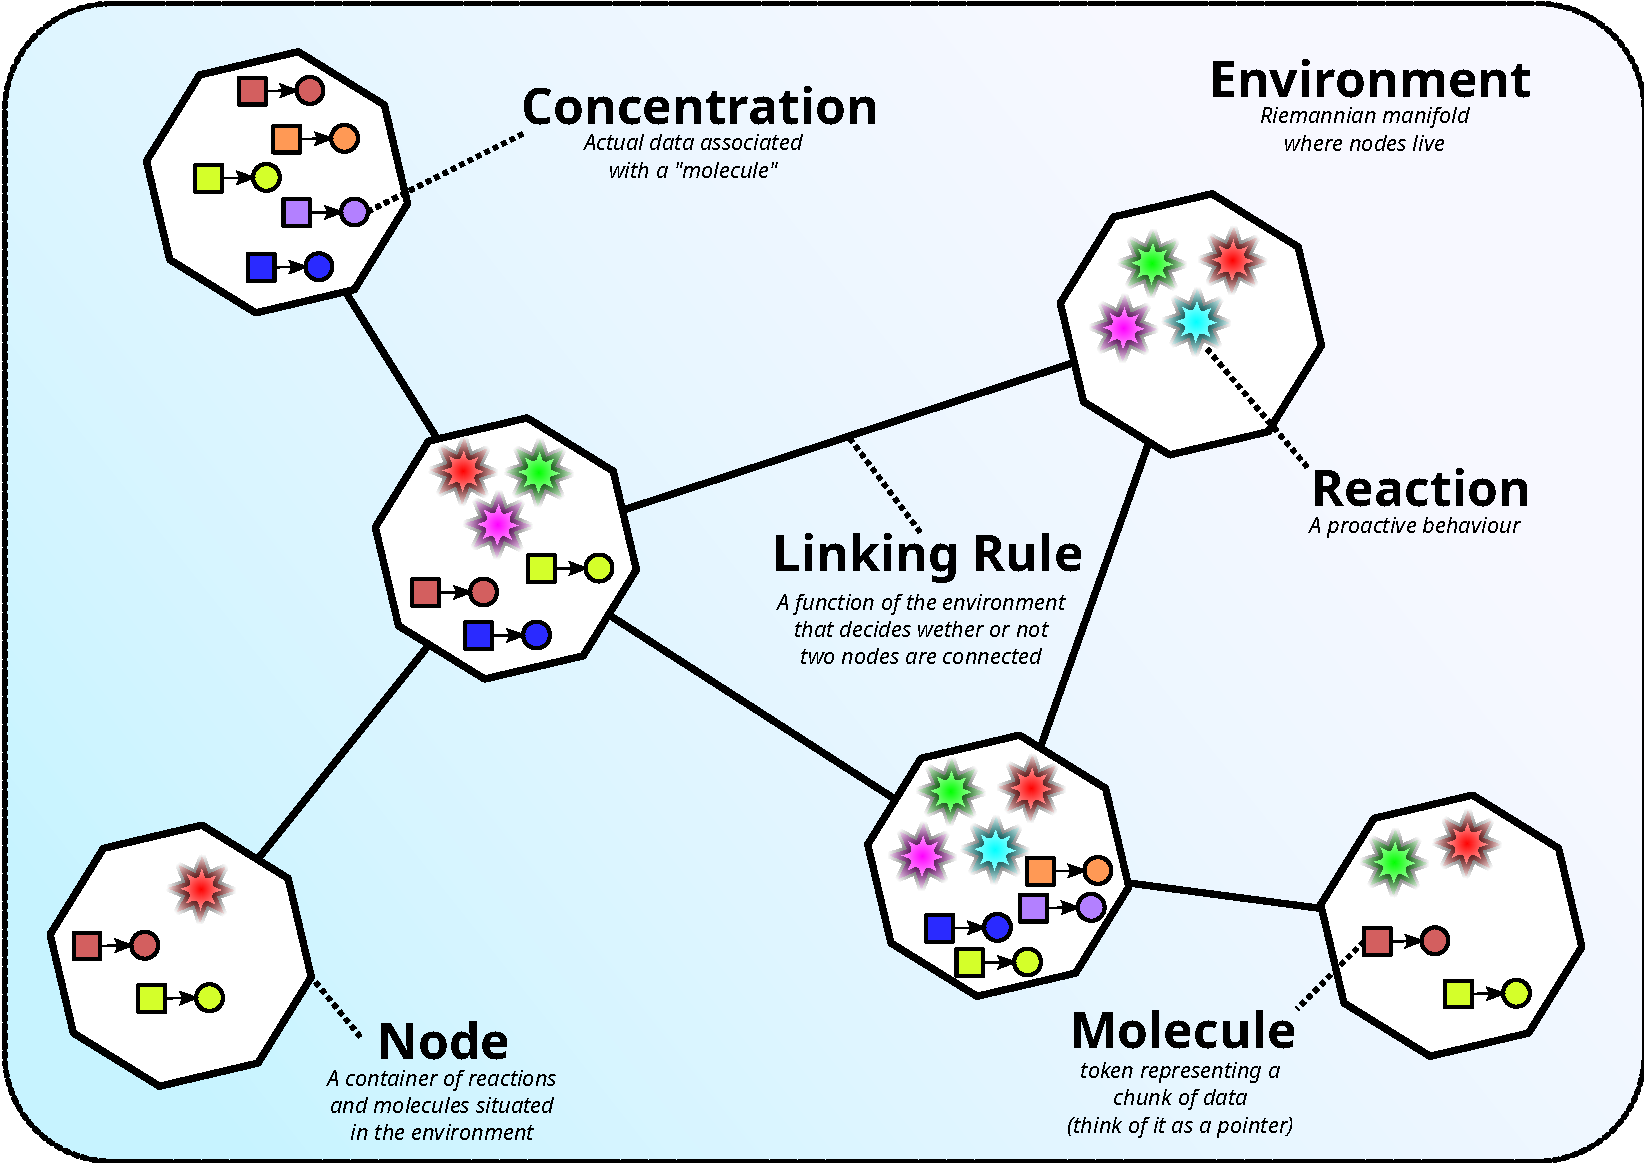
\includegraphics[width=\linewidth]{figures/AlchemistMetaModel.pdf}
    \caption{Rappresentazione grafica del meta-modello di Alchemist~\cite{pianini_2021}.}
    \label{fig:AlchemistMetaModel}
\end{figure}
\newpage

\subsubsection{Incarnazioni (\emph{Incarnations}) per Aggregate Programming}
\label{sec:incarnazioni}

Per supportare linguaggi e paradigmi differenti, Alchemist sfrutta il concetto di \emph{Incarnation} (incarnazione), che permette di definire il tipo di dato esatto usato per le variabili (Concentrazione) e di fornire comportamenti specifici~\cite{pianini_2021}. Tra le incarnazioni supportate, assumono particolare rilevanza: \texttt{collektive}, \texttt{protelis} e \texttt{scafi}. Queste incarnazioni sono progettate specificamente per eseguire programmi basati su \ac{AP}~\cite{pianini_2021}. Insieme, Alchemist e Collektive, consentono di implementare programmi aggregati in Kotlin che possono essere eseguiti e simulati in ambienti dinamici e configurabili~\cite{collektiveWeb}.

\subsubsection{Configurazione e Riproducibilità}
\label{sec:configurazione}

Alchemist semplifica la configurazione degli ambienti di test affidandosi a specifiche scritte in \emph{YAML}, un linguaggio di serializzazione dati in formato dichiarativo~\cite{pianini_2021}. Tramite un file YAML è possibile definire per esempio i modelli di rete (\emph{network-model}) e la disposizione iniziale dei nodi (\emph{deployments}). In \cref{lst:temperatureSimulation} viene mostrata la struttura di una possibile configurazione di una simulazione, riprendendo l'esempio: \cref{lst:exampleCollektive}.
\lstinputlisting[
float,
language=YAML,
label={lst:temperatureSimulation},
caption={Parte della configurazione della simulazione per il programma: \cref{lst:exampleCollektive}.}
]{listings/temperature.yml}
Un aspetto pratico fondamentale di Alchemist per le simulazioni in ambito marittimo è il supporto nativo a dati geospaziali. Il simulatore permette di importare ambienti fisici basati su OpenStreetMap e di impostare la dinamica dei nodi importando direttamente tracce \ac{GPS} in formato \ac{GPX} (generate, ad esempio, dalla decodifica di messaggi \ac{AIS}), consentendo di testare algoritmi sulle rotte effettivamente percorse dalle imbarcazioni~\cite{pianini_2021, 11217861}. Infine, Alchemist garantisce la ripetibilità degli esperimenti: il sistema separa e controlla in modo deterministico i seed (semi) dei generatori pseudo-casuali (come il Mersenne Twister) sia per la disposizione iniziale dei nodi, sia per l'esecuzione della simulazione~\cite{pianini_2021}.
\newpage

\section{Algoritmo precedente}
\label{sec:algoritmo_precedente}

L'esperimento su cui si basa questa tesi ha come obiettivo quello di migliorare la raccolta e la trasmissione di dati in uno scenario marittimo realistico. Il caso di studio considera il fiordo di Kiel, in Germania, dove le navi sono modellate come nodi in grado di comunicare tra loro e con stazioni a terra~\cite{11217861}. Il problema affrontato nasce dal divario tra la quantità di dati generata dai moderni sistemi di navigazione autonoma (\ac{MASS}) e la capacità delle infrastrutture di comunicazione marittima tradizionali. Navi autonome o semi-autonome possono infatti produrre flussi di dati ad alta intensità, derivanti ad esempio da telecamere e \ac{LiDAR}; al contrario, tecnologie tradizionali come \ac{AIS} e sistemi basati su \ac{VHF} offrono una capacità trasmissiva limitata~\cite{11217861}. Nella simulazione, ogni imbarcazione è dotata di diversi dispositivi di comunicazione: un sistema \ac{APRS} su \ac{VHF}, un dispositivo \ac{LoRaWAN} di classe C, un modulo 5G di tipo consumer e un dispositivo compatibile con Wi-Fi Direct~\cite{11217861}. Inoltre, alcune imbarcazioni possono essere equipaggiate con una torre 5G montata a bordo, con probabilità indicata dal parametro $p_{5G}$. Ogni nave tenta di trasmettere verso terra dei dati di dimensione fissata pari a $d = 3$~Mbit/s, valore scelto come approssimazione del bitrate necessario per un flusso video compresso a 720p~\cite{11217861}.

Per stimare la qualità dei collegamenti, l'esperimento associa a ogni coppia di nodi un data rate stimato in funzione della tecnologia disponibile e della distanza tra i dispositivi. Le tecnologie considerate sono quindi 5G, Wi-Fi, \ac{LoRaWAN} e \ac{APRS}. A partire da valori di riferimento ricavati dalla letteratura, il data rate in linea di vista viene stimato mediante interpolazione log-lineare rispetto alla distanza~\cite{11217861}.

Gli approcci confrontati nell'esperimento precedente sono quattro:
\begin{itemize}
    \item \emph{Baseline non cooperativa}: rappresenta lo stato dell'arte di riferimento. Ogni nave tenta di comunicare direttamente con una stazione a terra utilizzando la tecnologia più favorevole tra quelle disponibili. Se il collegamento diretto offre un data rate sufficiente a trasmettere il flusso $d$, la comunicazione viene considerata riuscita; in caso contrario, il flusso viene scartato~\cite{11217861}. Questo approccio non prevede alcuna collaborazione tra imbarcazioni.

    \item \emph{\ac{Dist-MR}}: ogni nave che non riesce a raggiungere direttamente la stazione a terra seleziona come relay un'imbarcazione vicina lungo il cammino geograficamente più breve verso la destinazione. Si ha quindi un insieme di alberi che originano nelle stazioni a terra. La metrica usata per la scelta del relay è la distanza geografica~\cite{11217861}.

    \item \emph{\ac{DR-MR}}: modifica il criterio di scelta del relay utilizzato in \ac{Dist-MR}. Invece di minimizzare la distanza geografica, l'obiettivo è selezionare il percorso che massimizza il data rate disponibile verso la stazione a terra~\cite{11217861}.

    \item \emph{\ac{CSC}}: organizza le imbarcazioni in cluster auto-organizzanti, la cui logica è implementata sfruttando la programmazione aggregata tramite il \ac{DSL} Collektive. Ogni cluster possiede un leader, responsabile della raccolta dei flussi dati prodotti dai membri della regione e della loro successiva sintesi prima dell'invio verso terra o verso un altro cluster. Questo approccio si basa sul pattern \ac{SCR}: i leader vengono eletti dinamicamente e la formazione dei cluster tiene conto della capacità di trasmettere dati verso il leader~\cite{11217861}.
\end{itemize}
